\graphicspath{{Images/}}

\section{Tester}

A partir do Tester corre um script a partir de um botão (figura 7). E mais 3 scripts quando se edita uma celula especifica (figura 8).
\subsection{Impressão de Escala}
Através do botão "TESTE" inicia-se o script "insertRow" (Tester 04 Get printTable) este script faz uma requisição externa HTTP GET. Esta função tem o proposito de premitir aos alunos de terem acesso à folha, enquanto o script corre. Caso isto não aconteça não seria possivel haver disposição das escalas nesta folha.

Através da função doGet é chamada a função "printTable" (Tester 04 printTable). Este script tem como objetivo mostrar quando é que o aluno irá fazer o seu próximo serviço. A primeira parte verifica se o aluno está a realizar uma troca, caso seja verdade, a escala será colocada na primeira tabela. Na segunda parte é verificado se há alguma troca ou não e consoante essa resposta a escala efetiva é colocada no primeiro local ou no segundo (fig.).

\subsection{Verificar}
Após colocar os NIP's para as trocas na tabela (O:P), na coluna "Verificar" (coluna Q), aparece uma checkbox na linha correspondente, quando esta é colocada em "true", é iniciado o script "SpecialOnEdit" (Tester 03 SpecialOnEdit). Dentro desta função é iniciado a função "check Editor" (Tester 03 check Editor) que verifica quem é o editor (é obrigatório o editor ser a pessoa com o NIP na coluna O).

Seguindo a função "SpecialOnEdit" (Tester 03 SpecialOnEdit) vai iniciar a função "verificarTroca1" (Tester 03 Get verificarTroca) esta vai fazer uma requisição "doGet" (Tester doGet) e de seguida iniciar a função "verificarTester" (Tester 03 verificarTroca). É nesta função que será verificada se a troca é possível.

Esta função está dividida em cinco grupos. O primeiro é a verificação de se os alunos estão de dispensa, o segundo verifica se os alunos estão a fazer troca e destroca na mesma escala, em terceiro lugar se a destroca acontece primeiro que a troca. Em qualquer um destes casos o programa não deixa avançar, caso estes problemas sejam verificados. O quarto grupo verifica se os alunos já estão a realizar uma troca, neste grupo, o programa avisa que o aluno já está a realizar a troca mas permite avançar para o envio do email. Por fim, o envio do email caso não se verifique nenhuma das verificações anteriores. Este email é enviado apenas para o aluno na coluna P através da função "emailSender" (Tester 03 Veri Troc emailer), nesta função são também protegidas as células das colunas O e P onde estão os NIPs dos alunos.

\subsection{Aceitar}
Após a verificação, na coluna "Aceitar" (coluna R), fica disponivel a checkbox. Colocando esta em "true", é iniciado "SpecialOnEdit" (Tester 03 SpecialOnEdit) e dentro desta "check Editor" (Tester 03 check Editor) em tudo semelhante ao "Verificar", (é obrigatório o editor ser a pessoa com o NIP na coluna P). De seguida é iniciado "troca" (Tester 02 Get aceitarTrocas) que irá fazer uma requisição "doGet" (Tester doGet) e de seguida iniciar a função "aceitarTrocas" (Tester 02 aceitarTrocas) que envia um email ao aluno na coluna O e para a secretaria.

\subsection{Secretaria}
Depois do envio do email, na coluna "Secretaria" (coluna S), fica disponivel a checkbox.Colocando esta em "true", é iniciado "SpecialOnEdit" (Tester 03 SpecialOnEdit). Esta coluna está apenas disponível para os editores (nomeadamente a secretaria). De seguida é iniciado "aceitarSec" (Tester 01 Get aceitarSec) que irá fazer uma requisição "doGet" (Tester doGet) e de seguida iniciar a função "aceitarSecretaria" (Tester 02 aceitarSec) que envia um email aos alunos na coluna O e P. Após o envio, coloca os NIPs na folha Geral, altera de "true" para "false" as três colunas e elimina-os da folha Tester. Retira a proteção das células onde estavam os NIPs.

    
    \begin{figure}[h!]
        \centering
        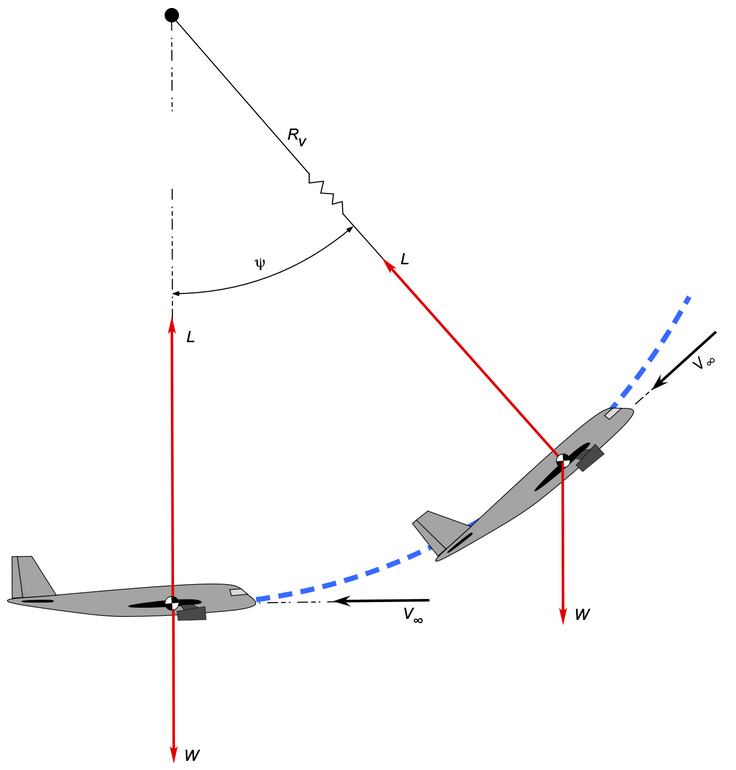
\includegraphics[width=.33\linewidth]{Imagens/img2_airPull.png}
        \caption{Somatório de forças em voo circular}
        \label{fig:enter-label}
    \end{figure}
    